\documentclass{article}

% TODO: please download neurips_2020.sty 
% from https://media.neurips.cc/Conferences/NeurIPS2020/Styles/neurips_2020.sty
% before building this document
\usepackage[preprint]{neurips_2020}

\usepackage[utf8]{inputenc} % allow utf-8 input
\usepackage[T1]{fontenc}    % use 8-bit T1 fonts
\usepackage{hyperref}       % hyperlinks
\usepackage{url}            % simple URL typesetting
\usepackage{booktabs}       % professional-quality tables
\usepackage{amsfonts}       % blackboard math symbols
\usepackage{nicefrac}       % compact symbols for 1/2, etc.
\usepackage{microtype}      % microtypography
\usepackage{graphicx}
\usepackage{amsthm}
\usepackage{amsmath}
\usepackage{bbm}
\usepackage{subfigure}

\newtheorem{theorem}{Theorem}

\title{Spectral clustering}

% The \author macro works with any number of authors. There are two commands
% used to separate the names and addresses of multiple authors: \And and \AND.
%
% Using \And between authors leaves it to LaTeX to determine where to break the
% lines. Using \AND forces a line break at that point. So, if LaTeX puts 3 of 4
% authors names on the first line, and the last on the second line, try using
% \AND instead of \And before the third author name.

\author{%
  Davide Riva \\
  \texttt{driva95@protonmail.com}
}

\begin{document}

\maketitle

\begin{abstract}
    The term "spectral clustering" refers to a series of unsupervised techniques to perform community detection in graphs using eigenvalues and eigenvectors.
    Even though there are some review articles about it, they usually have a lack of empirical analyses linked to the theoretical proofs.
    In this document, we are going to cover that part through experiments.
\end{abstract}

\section{Introduction}
Spectral clustering identifies communities inside a graph.
In Section \ref{section:twocom} we analyse how to extract communities in a noiseless scenario
in which there is only one connected component, identified as the only one community in the graph.
Then, Section \ref{section:multiplecom} considers multiple connected components and
Section \ref{section:noisecom} extends the previous ideas to a graph in which
the number of clusters is greater than the number of connected components.
Finally, Section \ref{section:nograph} explains how to use these techniques with data
which is not structured as a graph.

Note that every time we use the term "graph" we refer to undirected, weighted graphs
to avoid useless redundancy. All weights must be positive.

The experiments are written in Python in the form of Jupyter Notebooks
and they are provided together with this document as appendices.
The name of the used libraries and their version are also supplied through a \path{requirements.txt} file.

\section{Graphs with 1 connected component} \label{section:twocom}
We start by looking at a graph with a single connected component, as the one in Figure \ref{figure:plotga}.
We denote its weight matrix as $W \in \mathbb{R}^{n \times n}$.

\begin{figure}[hb]
    \hfill
    \subfigure[A graph with one connected component.]{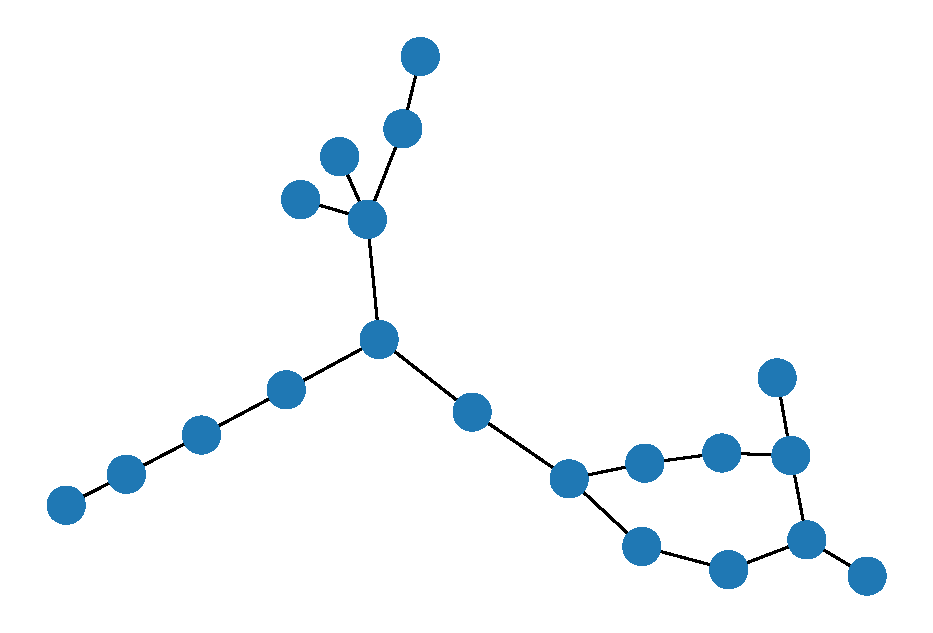
\includegraphics[width=0.5\linewidth]{figures/one-component.eps}}%
    \hfill
    \subfigure[A graph with three connected components.]{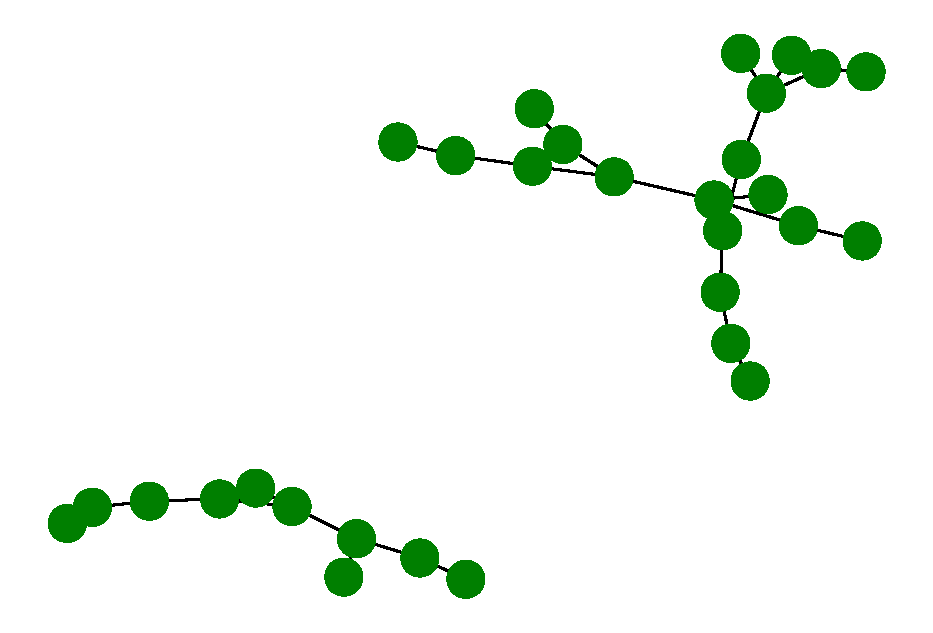
\includegraphics[width=0.5\linewidth]{figures/multiple-component.eps}}%
    \hfill
    \caption{Examples of graphs with various connected components.}%
    \label{figure:plotga}%
\end{figure}

The degree matrix $D$ of a graph is defined as a diagonal matrix whose diagonal elements are:
\begin{equation*}
    D_{ii} = \sum_{j=1}^n W_{ij}
\end{equation*}

The goal is to obtain an indicator vector $f = (f_1, \dots, f_n)$ which can identify which
node belongs to which connected component.
To do so, we build a matrix that we call Laplacian matrix:
\begin{equation*}
    L = D - W
\end{equation*}

\begin{theorem}
    Minimizing $\frac{1}{2} \sum_{i=1}^n \sum_{j=1}^n W_{ij} (f_i - f_j)$
    is equivalent to minimizing $f^T L f$.
\end{theorem}

\begin{proof}
    \begin{align*}
        f^T L f & = f^T D f - f^T W f                                                                                                 \\
                & = \sum_{i=1}^n D_{ii} f_i^2 - \sum_{i=1}^n \sum_{j=1}^n f_i f_j W_{ij}                                              \\
                & = \frac{1}{2} ( 2 \sum_{i=1}^n D_{ii} f_i^2 - 2 \sum_{i=1}^n \sum_{j=1}^n f_i f_j W_{ij})                           \\
                & = \frac{1}{2} ( \sum_{i=1}^n D_{ii} f_i^2 + \sum_{j=1}^n D_{jj} f_j^2 - 2 \sum_{i=1}^n \sum_{j=1}^n f_i f_j W_{ij}) \\
                & = \frac{1}{2} \sum_{i=1}^n \sum_{j=1}^n W_{ij} (f_i - f_j)^2 \tag*{\qedhere}
    \end{align*}
\end{proof}

We also know that $L$ is symmetric by definition. Furthermore, it is positive semi-definite since from the previous theorem
$f^T L f \geq 0 \; \forall f \in \mathbb{R}^n$.

It follows that the smallest eigenvalue of $L$ is 0. Its corresponding eigenvector is the vector $a [1, 1, \dots, 1], a \in \mathit{R}$
due to the fact that the sum of the elements of each row or column is always zero.
Note that if the graph has one connected component, the eigenvector corresponding to the eigenvalue with value 0 is the global minimum of the
minimization problem and a perfect solution for our task.

We can observe in an empirical way what we have just proved.
First, we generate a pre-defined number of graphs with one connected component.
In particular, each graph is a Watts–Strogatz model \cite{wc} which has the desired propriety of having a non-small clustering coefficient.
Then, we produce a box plot of the values of each eigenvalue sorted in ascending order for each graph.
The resulting plot can be seen in Figure \ref{figure:oneeigen}.

\begin{figure}[ht]
    \centering
    \includegraphics[width=0.5\linewidth]{figures/eigen-one-component.eps}
    \caption{Box plot of the eigenvalues of 100 graphs with 20 nodes and one connected component, sorted in ascending order for each graph.}
    \label{figure:oneeigen}
\end{figure}

\section{Graphs with multiple connected components} \label{section:multiplecom}
We now want to identify which node belongs to which connected component
when the graph has the number of connected components $k \geq 2$
as the one in Figure \ref{figure:plotga}.

First, we rearrange the matrix $L$ grouping together nodes in the same connected component.
In this way, $L$ is a block diagonal matrix with subgraphs $L_1, \dots, L_k$.
Now, each subgraph has one and only one connected component
and therefore it has one eigenvalue that is equal to zero,
as proven in Section \ref{section:twocom}.

We also know from linear algebra that the set of eigenvalues of $L$
is composed of the eigenvalues of $L_1, \dots, L_k$.
Also, each corresponding eigenvector in $L_i$ is a valid eigenvector in $L$ with zero padding
in the other block positions.
It follows that the matrix $L$ has $k$ eigenvalues with value equals to zero and
one combination of eigenvalues valid in that eigenspace is composed of indicator vectors.
This propriety can be seen empirically in Figure \ref{figure:mcomp},
where each graph is again a Watts–Strogatz model.

\begin{figure}[hb]
    \hfill
    \subfigure[Graphs with two connected components.]{\includegraphics[width=0.3\linewidth]{figures/2-components.eps}}
    \hfill
    \subfigure[Graphs with four connected components.]{\includegraphics[width=0.3\linewidth]{figures/4-components.eps}}
    \hfill
    \subfigure[Graphs with eight connected components.]{\includegraphics[width=0.3\linewidth]{figures/8-components.eps}}
    \hfill
    \label{figure:mcomp}
    \caption{Box plot of the first 10 eigenvalues of 100 graphs with 64 nodes and different connected components, sorted in ascending order for each graph.}
\end{figure}

Since in this scenario the eigenspace of the eigenvalues with value zero
is a linear combination of indicator vectors, we use them to identify the connected components.
In particular, we build a matrix $V \in \mathit{R}^{n \times k}$ where each column corresponds to
an eigenvector of the previous eigenspace.
Finally, K-means is performed over the matrix $V$ to group data,
since groups in $V$ are linearly separable.

In order to see if the eigenvectors described before are good indicator vectors,
we build a graph with three connected components:
the first cluster corresponds to the first three nodes,
the second cluster is composed of the last two and the third has all the remaining ones.
Each connected component of the graph is a complete graph itself.
Figure \ref{figure:eivects} represents this configuration graphically.

\begin{figure}[hb]
    \hfill
    \subfigure{\includegraphics[width=0.3\linewidth]{figures/0-eigenvectors.eps}}%
    \hfill
    \subfigure{\includegraphics[width=0.3\linewidth]{figures/1-eigenvectors.eps}}%
    \hfill
    \subfigure{\includegraphics[width=0.3\linewidth]{figures/2-eigenvectors.eps}}%
    \hfill
    \caption{Example of eigenvectors used as indicator vectors.}%
    \label{figure:eivects}%
\end{figure}

\section{Considerations about noise} \label{section:noisecom}
Until now we considered the situation in which each detected community
corresponds to a connected component of the graph.

If we instead assume that each cluster is a tightly coupled group of nodes
with a low number of inter-community edges, we can treat these edges as noise added
to the situations described in the previous sections.
Given the noiseless adjacency matrix $A$,
we can view the edges presented before as a perturbation $H$ that produces the final
matrix $W = A + H$.

Thanks to the Davis–Kahan theorem \cite{davis1970rotation} we can state that small perturbations
in the Laplacian matrix lead to small perturbations in its eigenvectors and eigenvalues.
This means that if the noise (in our case, the addition of unwanted edges) is small,
it is still possible to perform spectral clustering.
In particular, we choose the number of communities looking at each eigengap:
small eigengaps are considered produced by noise,
while the first eigengap greater than the previous ones is assumed to be the dividing
indicator between eigenvectors used as indicator vectors and other eigenvectors.
Using the eigengap as a criterion to decide the number of communities in a graph
can be justified in other ways, well documented in \cite{DBLP:journals/corr/abs-0711-0189}.

To empirically verify the quality of using the eigengap to identify the number of clusters,
we start from a graph composed of three connected components which are complete graphs themselves and
we add iteratively more edges until all nodes are connected to all the others.
As we can see from Figure \ref{figure:addingnoise}:
\begin{itemize}
    \item The smallest eigenvalue is zero all the time since there is always at least one connected component in a graph.
    \item The first three eigenvalues in ascending order are initially zero when there is no noise and then they grow when edges are added.
    \item The eigengap between the third and the fourth eigenvalue is bigger than the others until there is too much noise.
\end{itemize}

\begin{figure}[ht]
    \centering
    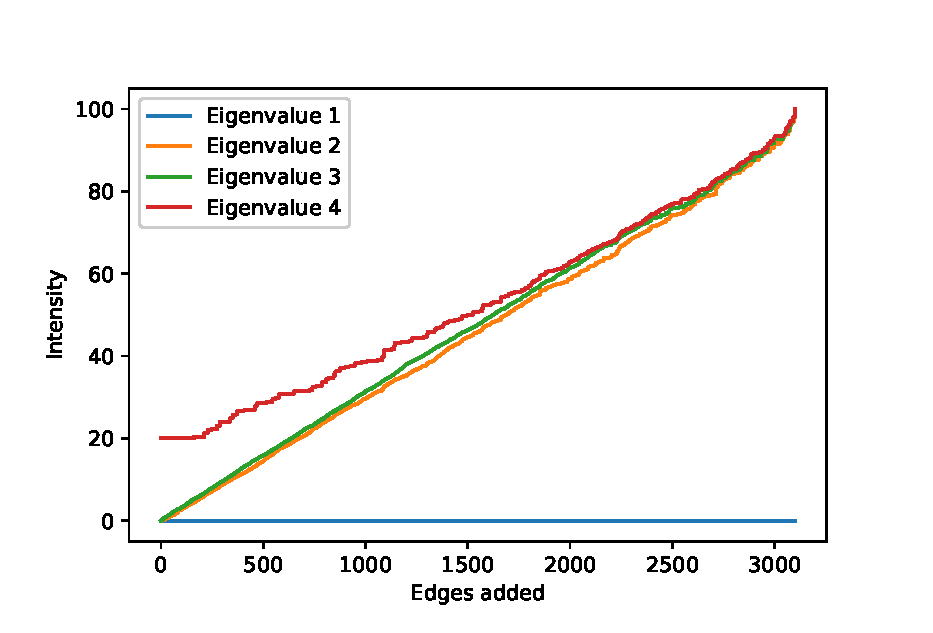
\includegraphics[width=0.5\linewidth]{figures/adding-noise.eps}
    \caption{Example of the effect of noise in the eigenvalues intensities in a graph with 3 connected components.}
    \label{figure:addingnoise}
\end{figure}


\section{Spectral clustering when data is not a graph} \label{section:nograph}
We have previously seen how to use spectral clustering to identify communities in graphs.
In this section, we extend this concept to a set of data points $x_1, x_2, \dots, x_n$.

First, we introduce the family of similarity functions $s(x_i, x_j) \geq 0$ which can be used to build an adjacency matrix.
$s(x_i, x_j)$ can be defined in a lot of ways, for instance:
\begin{itemize}
    \item $s(x_i, x_j) = e^{ - \frac{||x_i - x_j||^2}{2\sigma^2}}$ (Gaussian similarity function): it produces a graph in which all nodes are connected with each other, but everyone with different weights.
    \item $s(x_i, x_j) = ||x_i - x_j||_2 < \epsilon$: it produces an unweighted graph.
    \item $s(x_i, x_j) = \frac{1}{\sqrt{2}} \sqrt{\sum_k (\sqrt{x_i(k)} - \sqrt{x_j(k)})^2}$ (Hellinger distance \cite{PPN243919689_0136}): useful when each data point is a discrete probability distribution.
\end{itemize}

Then, we perform spectral clustering using the adjacency matrix built before.
As previously mentioned, thanks to this technique it is possible to perform clustering in situations in which
clusters are not linearly separable.

To compare it with K-means, we generate some synthetic data.
During this experiment, spectral clustering uses $s(x_i, x_j) = ||x_i - x_j||_2 < \epsilon$ as a similarity function.
Figure \ref{figure:comparison} shows the dataset generated and the best results obtained with these two methods.
Clearly, spectral clustering outperforms K-means.

\begin{figure}[ht]
    \hfill
    \subfigure[Ground truth.]{\includegraphics[width=0.3\linewidth]{figures/ground-truth.eps}}%
    \hfill
    \subfigure[Clustering using K-means.]{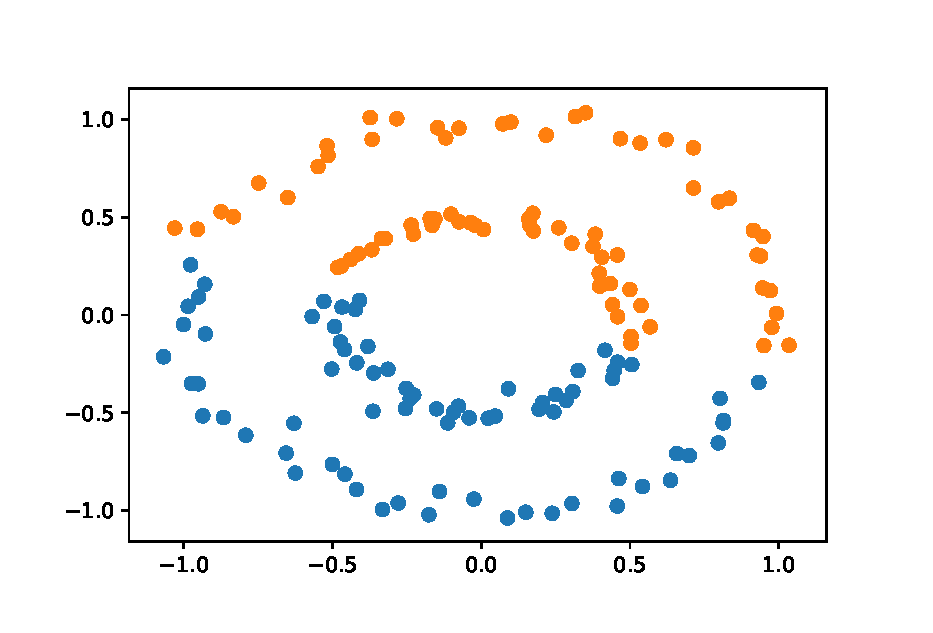
\includegraphics[width=0.3\linewidth]{figures/kmeans.eps}}%
    \hfill
    \subfigure[Clustering using spectral clustering.]{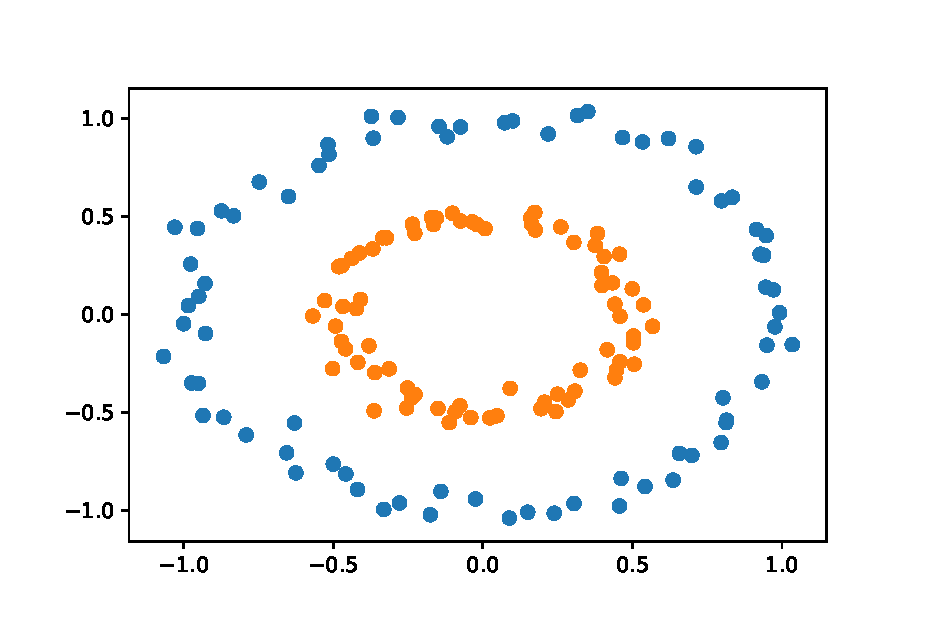
\includegraphics[width=0.3\linewidth]{figures/spectral-on-comparison.eps}}%
    \hfill
    \caption{Comparison between K-means and spectral clustering.}%
    \label{figure:comparison}%
\end{figure}

So far we have manually tweaked the hyperparameter $\epsilon$ and the number of clusters to find the best solution for each dataset.
We now ask ourselves if there is a way to automatically choose the right value for them.
To do so, we introduce the modularity quality function (presented in \cite{fortunato2010community}):
\begin{equation*}
    Q = \frac{1}{2m} \sum_{i=1}^n \sum_{j=1}^n (A_{ij} - \frac{k_i k_j}{2m}) \mathbbm{1}_{[C_i == C_j]}
\end{equation*}
where $m$ is the number of edges of the unweighted graph for which the modularity is computed,
$A$ is the adjacency matrix,
$k_i$ is the degree of the node $i$
and $C_i$ the index of the connected component of the node $i$.
This function measures how different the considered unweighted graph is from a graph with the same degree sequence but with
edges connected randomly.  High values of modularity correspond to the presence of clusters;
vice versa low modularity suggests a graph without sharp partitions.

Since binarizing the graph produces multiple connected components if the threshold is chosen through modularity,
we hypothesize is that it might help spectral clustering.
To empirically test our idea, we use the "Mall customers" dataset.\footnote{\url{https://www.kaggle.com/kandij/mall-customers}}
We then compute the modularity with 100 different thresholds and we pick the largest threshold between the ones with high modularity.
Looking at the eigenvalues near zero, we identify 57 clusters.
We then perform spectral clustering considering true the number of clusters found.
The previous steps are then compared with spectral clustering using the Gaussian similarity function manually tweaking the number of clusters
and the $\sigma$ parameter. As we can see from Figure \ref{figure:realworld},
manually tweaking the hyperparameters outperforms our results.
Looking at the literature, \cite{DBLP:journals/corr/abs-0711-0189} founds no theoretical justification in different methods proposed to overcome this issue.
Since the cited review article is from 2007, we searched in the literature but without finding anything useful from a theoretical point of view.

\begin{figure}[hb]
    \hfill
    \subfigure[Raw data.]{\includegraphics[width=0.3\linewidth]{figures/mall-raw.png}}%
    \hfill
    \subfigure[Spectral clustering with modularity.]{\includegraphics[width=0.3\linewidth]{figures/mall-spectral.png}}%
    \hfill
    \subfigure[Spectral clustering.]{\includegraphics[width=0.3\linewidth]{figures/mall-manual.png}}%
    \hfill
    \caption{Comparison between spectral clustering using the Gaussian similarity function and spectral clustering using modularity first.}%
    \label{figure:realworld}%
\end{figure}

\pagebreak
\nocite{*}
\bibliography{references}
\bibliographystyle{plain}

\end{document}